\documentclass[11pt,preprint, authoryear]{elsarticle}

\usepackage{lmodern}
%%%% My spacing
\usepackage{setspace}
\setstretch{1.2}
\DeclareMathSizes{12}{14}{10}{10}

% Wrap around which gives all figures included the [H] command, or places it "here". This can be tedious to code in Rmarkdown.
\usepackage{float}
\let\origfigure\figure
\let\endorigfigure\endfigure
\renewenvironment{figure}[1][2] {
    \expandafter\origfigure\expandafter[H]
} {
    \endorigfigure
}

\let\origtable\table
\let\endorigtable\endtable
\renewenvironment{table}[1][2] {
    \expandafter\origtable\expandafter[H]
} {
    \endorigtable
}


\usepackage{ifxetex,ifluatex}
\usepackage{fixltx2e} % provides \textsubscript
\ifnum 0\ifxetex 1\fi\ifluatex 1\fi=0 % if pdftex
  \usepackage[T1]{fontenc}
  \usepackage[utf8]{inputenc}
\else % if luatex or xelatex
  \ifxetex
    \usepackage{mathspec}
    \usepackage{xltxtra,xunicode}
  \else
    \usepackage{fontspec}
  \fi
  \defaultfontfeatures{Mapping=tex-text,Scale=MatchLowercase}
  \newcommand{\euro}{€}
\fi

\usepackage{amssymb, amsmath, amsthm, amsfonts}

\def\bibsection{\section*{References}} %%% Make "References" appear before bibliography


\usepackage[round]{natbib}

\usepackage{longtable}
\usepackage[margin=2.3cm,bottom=2cm,top=2.5cm, includefoot]{geometry}
\usepackage{fancyhdr}
\usepackage[bottom, hang, flushmargin]{footmisc}
\usepackage{graphicx}
\numberwithin{equation}{section}
\numberwithin{figure}{section}
\numberwithin{table}{section}
\setlength{\parindent}{0cm}
\setlength{\parskip}{1.3ex plus 0.5ex minus 0.3ex}
\usepackage{textcomp}
\renewcommand{\headrulewidth}{0.2pt}
\renewcommand{\footrulewidth}{0.3pt}

\usepackage{array}
\newcolumntype{x}[1]{>{\centering\arraybackslash\hspace{0pt}}p{#1}}

%%%%  Remove the "preprint submitted to" part. Don't worry about this either, it just looks better without it:
\makeatletter
\def\ps@pprintTitle{%
  \let\@oddhead\@empty
  \let\@evenhead\@empty
  \let\@oddfoot\@empty
  \let\@evenfoot\@oddfoot
}
\makeatother

 \def\tightlist{} % This allows for subbullets!

\usepackage{hyperref}
\hypersetup{breaklinks=true,
            bookmarks=true,
            colorlinks=true,
            citecolor=blue,
            urlcolor=blue,
            linkcolor=blue,
            pdfborder={0 0 0}}


% The following packages allow huxtable to work:
\usepackage{siunitx}
\usepackage{multirow}
\usepackage{hhline}
\usepackage{calc}
\usepackage{tabularx}
\usepackage{booktabs}
\usepackage{caption}


\newenvironment{columns}[1][]{}{}

\newenvironment{column}[1]{\begin{minipage}{#1}\ignorespaces}{%
\end{minipage}
\ifhmode\unskip\fi
\aftergroup\useignorespacesandallpars}

\def\useignorespacesandallpars#1\ignorespaces\fi{%
#1\fi\ignorespacesandallpars}

\makeatletter
\def\ignorespacesandallpars{%
  \@ifnextchar\par
    {\expandafter\ignorespacesandallpars\@gobble}%
    {}%
}
\makeatother

\newenvironment{CSLReferences}[2]{%
}

\urlstyle{same}  % don't use monospace font for urls
\setlength{\parindent}{0pt}
\setlength{\parskip}{6pt plus 2pt minus 1pt}
\setlength{\emergencystretch}{3em}  % prevent overfull lines
\setcounter{secnumdepth}{5}

%%% Use protect on footnotes to avoid problems with footnotes in titles
\let\rmarkdownfootnote\footnote%
\def\footnote{\protect\rmarkdownfootnote}
\IfFileExists{upquote.sty}{\usepackage{upquote}}{}

%%% Include extra packages specified by user

%%% Hard setting column skips for reports - this ensures greater consistency and control over the length settings in the document.
%% page layout
%% paragraphs
\setlength{\baselineskip}{12pt plus 0pt minus 0pt}
\setlength{\parskip}{12pt plus 0pt minus 0pt}
\setlength{\parindent}{0pt plus 0pt minus 0pt}
%% floats
\setlength{\floatsep}{12pt plus 0 pt minus 0pt}
\setlength{\textfloatsep}{20pt plus 0pt minus 0pt}
\setlength{\intextsep}{14pt plus 0pt minus 0pt}
\setlength{\dbltextfloatsep}{20pt plus 0pt minus 0pt}
\setlength{\dblfloatsep}{14pt plus 0pt minus 0pt}
%% maths
\setlength{\abovedisplayskip}{12pt plus 0pt minus 0pt}
\setlength{\belowdisplayskip}{12pt plus 0pt minus 0pt}
%% lists
\setlength{\topsep}{10pt plus 0pt minus 0pt}
\setlength{\partopsep}{3pt plus 0pt minus 0pt}
\setlength{\itemsep}{5pt plus 0pt minus 0pt}
\setlength{\labelsep}{8mm plus 0mm minus 0mm}
\setlength{\parsep}{\the\parskip}
\setlength{\listparindent}{\the\parindent}
%% verbatim
\setlength{\fboxsep}{5pt plus 0pt minus 0pt}



\begin{document}



\begin{frontmatter}  %

\title{Question 5}

% Set to FALSE if wanting to remove title (for submission)




\author[Add1]{Peter Meihuizen}
\ead{21831041@sun.ac.za}





\address[Add1]{Stellenbosch University}



\vspace{1cm}


\begin{keyword}
\footnotesize{
Multivariate GARCH \sep Kalman Filter \sep Copula \\
\vspace{0.3cm}
}
\footnotesize{
\textit{JEL classification} L250 \sep L100
}
\end{keyword}



\vspace{0.5cm}

\end{frontmatter}

\setcounter{footnote}{0}



%________________________
% Header and Footers
%%%%%%%%%%%%%%%%%%%%%%%%%%%%%%%%%
\pagestyle{fancy}
\chead{}
\rhead{}
\lfoot{}
\rfoot{\footnotesize Page \thepage}
\lhead{}
%\rfoot{\footnotesize Page \thepage } % "e.g. Page 2"
\cfoot{}

%\setlength\headheight{30pt}
%%%%%%%%%%%%%%%%%%%%%%%%%%%%%%%%%
%________________________

\headsep 35pt % So that header does not go over title




\hypertarget{introduction}{%
\section{\texorpdfstring{Introduction
\label{Introduction}}{Introduction }}\label{introduction}}

For this question we will be looking at the database of app downloads
from Google to see what encourages people to download a particular app.

\hypertarget{analysis}{%
\section{\texorpdfstring{Analysis
\label{Analysis}}{Analysis }}\label{analysis}}

Firstly I need to import the data.

Ok so based on the data I want to see what are the most downloaded types
of apps, therefore I will look at the median number of downloads per
application type. First I need to change this line to be numeric values.

Ok so now I want to see which app categories are the most used. In order
to do that I am going to do a scatter plot which shows the average
number of reviews of each app category, as well as the average number of
downloads received by each category.

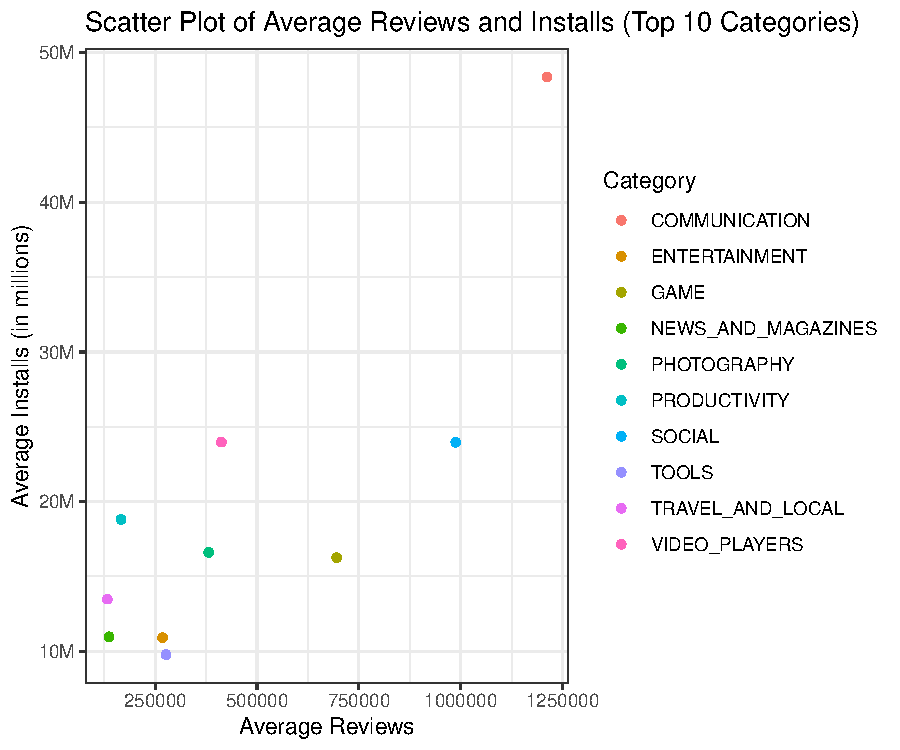
\includegraphics{Question_5_files/figure-latex/unnamed-chunk-3-1.pdf}

Ok so we can see that communication apps are by far the most installed
type of app on average, having the highest average number of reviews and
installations. In terms of installations it is followed by social apps
and then gaming apps. The second most reviewed category seems to be
video\_players.

So we know what is the most used types of apps and most reviewed.
However an important factor when understanding the reviews of a
particular is app is whether or not they are positive. Apps with more
positive reviews are likely to be used more frequently, so using the
user review data set, we can compare the percentage of positive,
negative and neutral reviews for each app category.

Ok now we must merge the category column to be assigned with
therespective app in the Review data set.

Ok so now using the merged data we can work out the percentage of each
type of review in each category.

\begin{verbatim}
## # A tibble: 10 x 4
##    Category           pos_percent neg_percent neu_percent
##    <chr>                    <dbl>       <dbl>       <dbl>
##  1 COMMUNICATION             62.7        20.6       16.7 
##  2 ENTERTAINMENT             58.3        25.5       16.2 
##  3 GAME                      58.1        37.5        4.37
##  4 NEWS_AND_MAGAZINES        57.6        29.3       13.1 
##  5 PHOTOGRAPHY               65.7        20.4       13.9 
##  6 PRODUCTIVITY              68.8        18.7       12.4 
##  7 SOCIAL                    54.1        26.2       19.7 
##  8 TOOLS                     60.4        17.6       22.0 
##  9 TRAVEL_AND_LOCAL          60.9        21.3       17.8 
## 10 VIDEO_PLAYERS             57.4        25.1       17.5
\end{verbatim}

So as can be seen most app categories have round 60\% positive reviews,
25\% negative reviews and 15\% neutral reviews. Communication apps have
a good positive percentage relative to other app types. They have the
best percentage results amongst their closest competitors in terms of
installations, with 63\% positive reviews and 21\% negative reviews.
Comparatively, social apps having 54\% positive reviews and 26\%
negative reviews, whilst gaming apps have 58\% positive reviews and 37\%
negative reviews. Based on these results it seems evident that the best
type of app to produce would be a Communication app.

\bibliography{Tex/ref}





\end{document}
